\section{Данные и EDA}

\subsection{Источник данных}
Используется датасет CIFAR-10 (10 классов, изображения $32 \times 32$).

\subsection{EDA, релевантный задаче ЛР}
Для данной ЛР основной акцент не на табличном EDA, а на:
\begin{itemize}
    \item сбалансированности классов;
    \item визуальной проверке качества входных изображений;
    \item статистике значений пикселей после преобразований.
\end{itemize}

\begin{figure}[H]
    \centering
    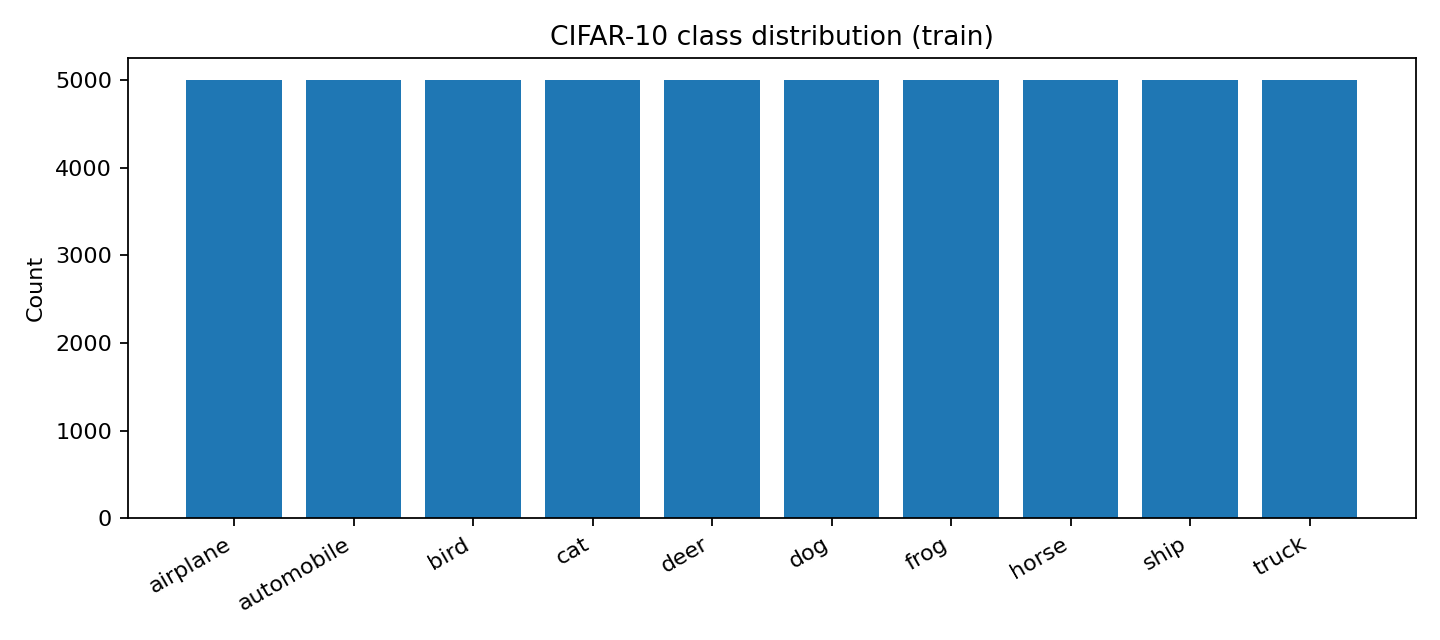
\includegraphics[width=0.75\textwidth]{figures/eda_class_distribution.png}
    \caption{Распределение классов в train-части CIFAR-10.}
    \label{fig:eda_class_dist}
\end{figure}

\begin{figure}[H]
    \centering
    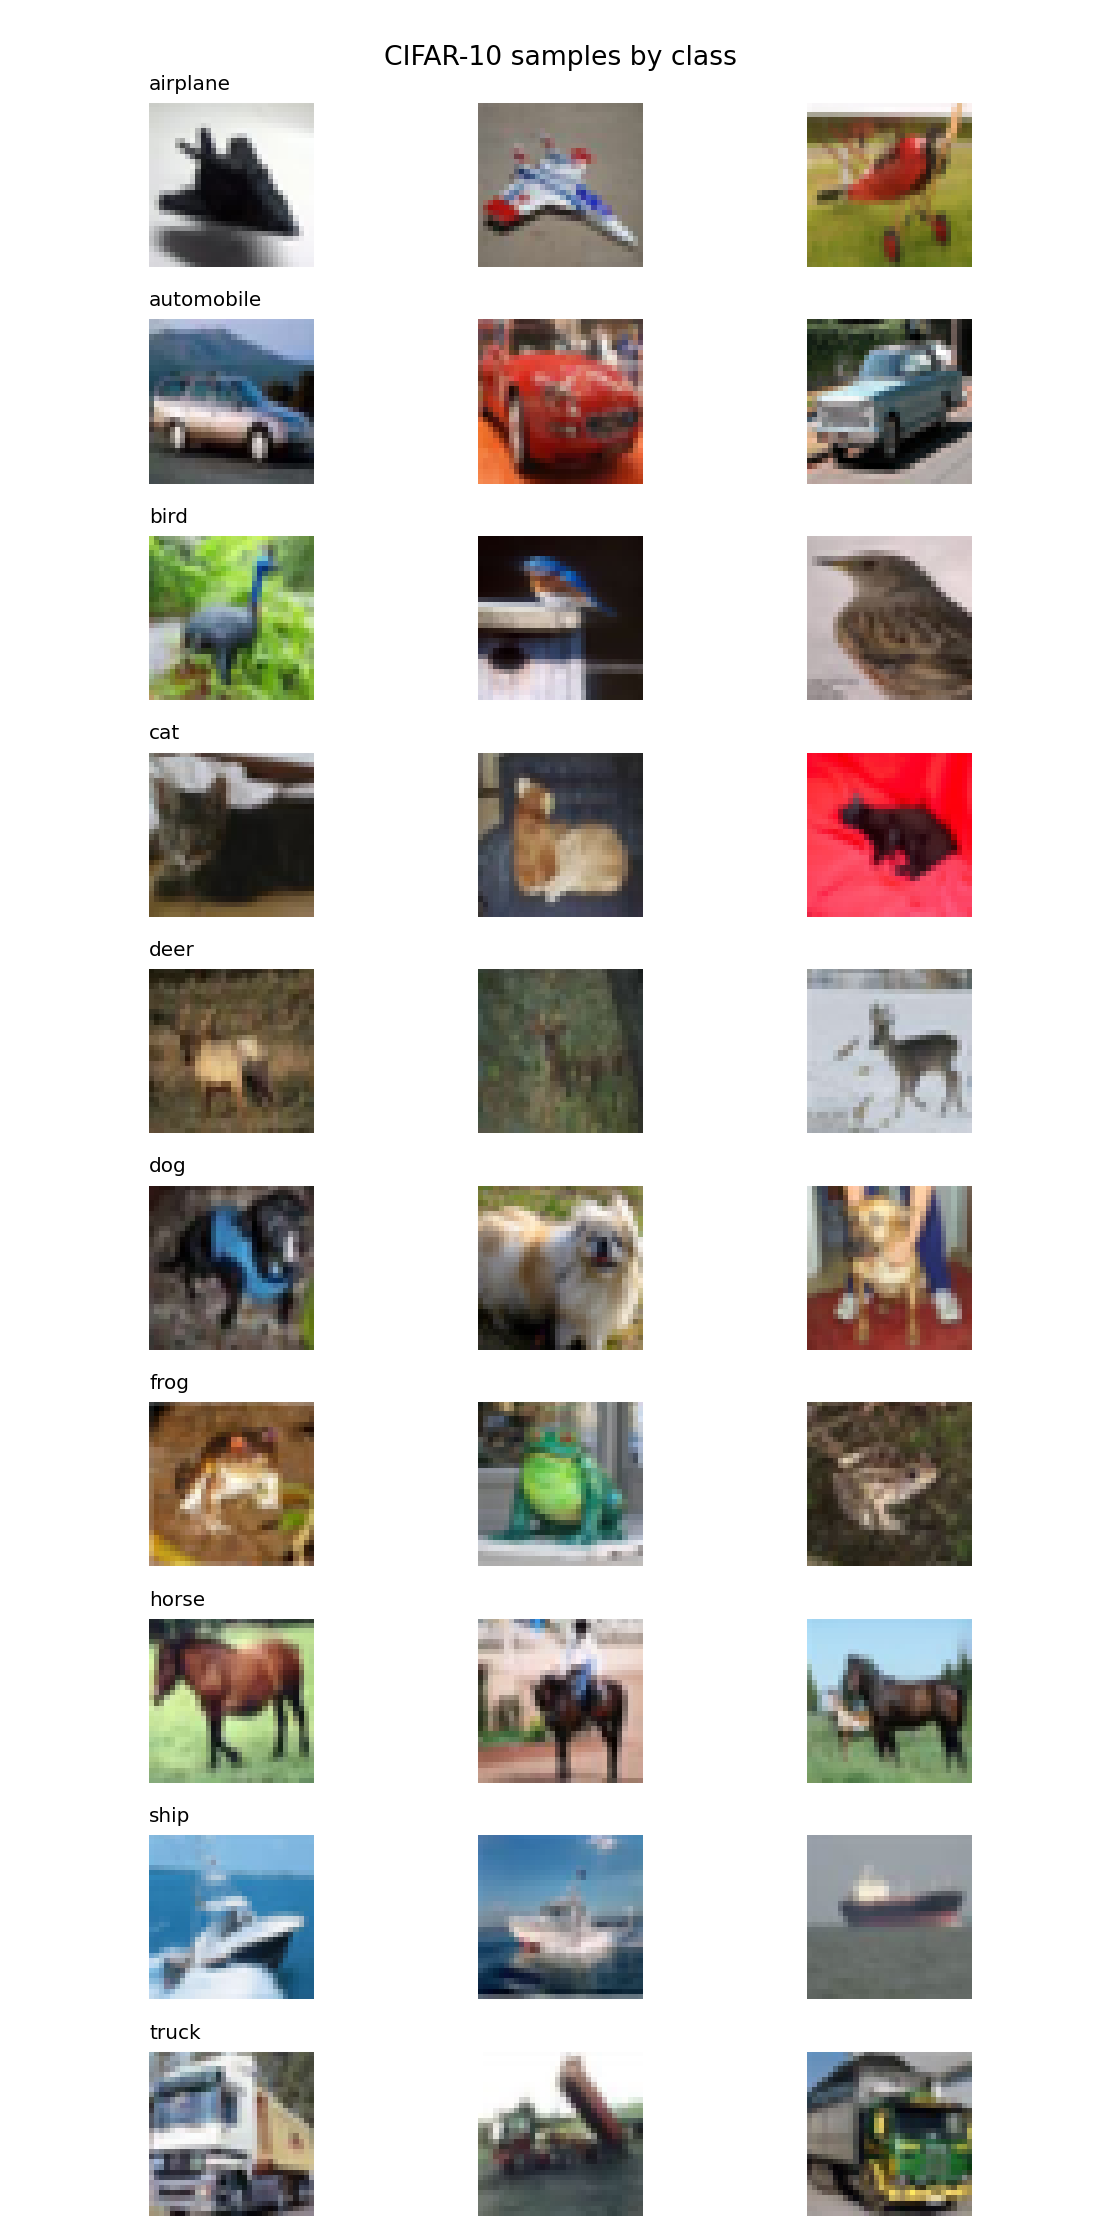
\includegraphics[width=\textwidth]{figures/eda_sample_grid.png}
    \caption{Примеры изображений CIFAR-10 (по одному/нескольким образцам классов).}
    \label{fig:eda_sample_grid}
\end{figure}

\subsection{Интерпретация}
Сбалансированность классов снижает риск смещения метрик из-за class imbalance. Для нашей задачи это важно, так как вариации в landscape должны объясняться геометрией loss и архитектурой, а не перекосом выборки.
